%    Copyright (C) 2012  L. Schmid
%
%    This file is free: you can redistribute it and/or modify
%    it under the terms of the GNU General Public License as published by
%    the Free Software Foundation, either version 3 of the License, or
%    (at your option) any later version, but you have to reference to the original owner.
%
%	 Additionaly the authors have to be readable in the final document.
%
%    This program is distributed in the hope that it will be useful,
%    but WITHOUT ANY WARRANTY; without even the implied warranty of
%    MERCHANTABILITY or FITNESS FOR A PARTICULAR PURPOSE.  See the
%    GNU General Public License for more details.
%
%    You should have received a copy of the GNU General Public License
%    along with this program.  If not, see <http://www.gnu.org/licenses/>.

%%%%%%%%%%%%%%%%%%%%%%%%%
% Dokumentinformationen %
%%%%%%%%%%%%%%%%%%%%%%%%%
\newcommand{\titleinfo}{Partielle Differential Gleichungen}
\newcommand{\authorinfo}{L.Schmid}
\newcommand{\versioninfo}{$Revision:  $ - powered by \LaTeX}

%%%%%%%%%%%%%%%%%%%%%%%%%%%%%%%%%%%%%%%%%%%%%
% Standard projekt�bergreifender Header f�r
% - Makros 
% - Farben
% - Mathematische Operatoren 
%
% DORT NUR ERG�NZEN, NICHTS L�SCHEN
%%%%%%%%%%%%%%%%%%%%%%%%%%%%%%%%%%%%%%%%%%%%%  
% Genereller Header
\documentclass[10pt,twoside,a4paper,fleqn]{article}
\usepackage[utf8]{inputenc}
\usepackage[left=1cm,right=1cm,top=1cm,bottom=1cm,includeheadfoot]{geometry}
\usepackage[ngerman]{babel,varioref}
\usepackage[T1]{fontenc}

% Pakete
\usepackage{amssymb}
\usepackage{amsmath}
\usepackage{bm} %bold math symbols
\usepackage{fancybox}
\usepackage{graphicx}
\usepackage{color}
\usepackage{xcolor}
\usepackage{lastpage}
\usepackage{wrapfig}
\usepackage{fancyhdr}
\usepackage{hyperref}
\usepackage{verbatim}
\usepackage{floatflt}
\usepackage{arydshln}
\usepackage{ucs}
\usepackage{pdflscape} % landscape
\usepackage{multirow} % zellen in tabellen verbinden
\usepackage{multicol} 
%s\usepackage{diagbox} % getrennte zelle in tabelle
% \usepackage{array} % anordnung in tabellen

%%%%%%%%%%%%%%%%%%%%
% Generelle Makros %
%%%%%%%%%%%%%%%%%%%%
\newcommand{\formelbuch}[1]{$_{\textcolor{red}{\mbox{\small{S#1}}}}$}
\newcommand{\verweis}[2]{ {\small (siehe auch \ref{#1}, #2 (S. \pageref{#1}))
}}
\newcommand{\subsubadd}[1]{\textcolor{black}{\mbox{#1}}}
\newenvironment{liste}[0]{
	\begin{list}{$\bullet$}{\setlength{\itemsep}{0cm}\setlength{\parsep}{0cm} \setlength{\topsep}{0cm}}}
    {\end{list}}
    
\newcommand{\logd}[0]{\log_{10}}
\newcommand{\subsubsubsection}[1]{\textbf{#1}}

\newenvironment{aufzaehlung}[0]{
	\begin{enumerate}{\setlength{\itemsep}{0cm}\setlength{\parsep}{0cm}
	\setlength{\topsep}{0cm}}} {\end{enumerate}}    

\newcommand{\abbHeight}[3]{
	\begin{center}
		\includegraphics[height=#2]{./bilder/#1} \\
		#3
    \end{center}
}

%\newcommand{\skriptsection}[2]{\section{#1 {\tiny Skript S. #2}}}
%\newcommand{\skriptsubsection}[2]{\subsection{#1 {\tiny Skript S. #2}}}
%\newcommand{\skriptsubsubsection}[2]{\subsubsection{#1 {\tiny Skript S. #2}}}
%\renewcommand{\skriptsection}[2]{\section{#1 {\tiny Schaum S. #2}}}
%\renewcommand{\skriptsubsection}[2]{\subsection{#1 {\tiny Schaum S. #2}}}
%\renewcommand{\skriptsubsubsection}[2]{\subsubsection{#1 {\tiny Schaum S. #2}}}
\newcommand{\skriptsection}[2]{\section{#1 \formelbuch{#2}}}
\newcommand{\skriptsubsection}[2]{\subsection{#1 \formelbuch{#2}}}
\newcommand{\skriptsubsubsection}[2]{\subsubsection{#1 \formelbuch{#2}}}

%%%%%%%%%%
% Farben %
%%%%%%%%%%
\definecolor{black}{rgb}{0,0,0}
\definecolor{red}{rgb}{1,0,0}
\definecolor{white}{rgb}{1,1,1}
\definecolor{grey}{rgb}{0.8,0.8,0.8}

%%%%%%%%%%%%%%%%%%%%%%%%%%%%
% Mathematische Operatoren %
%%%%%%%%%%%%%%%%%%%%%%%%%%%%
\DeclareMathOperator{\sinc}{sinc}
\DeclareMathOperator{\sgn}{sgn}
\DeclareMathOperator{\tr}{tr}
\DeclareMathOperator{\tridiag}{tridiag}



% Fouriertransformationen
\unitlength1cm
\newcommand{\FT}
{
\begin{picture}(1,0.5)
\put(0.2,0.1){\circle{0.14}}\put(0.27,0.1){\line(1,0){0.5}}\put(0.77,0.1){\circle*{0.14}}
\end{picture}
}


\newcommand{\IFT}
{
\begin{picture}(1,0.5)
\put(0.2,0.1){\circle*{0.14}}\put(0.27,0.1){\line(1,0){0.45}}\put(0.77,0.1){\circle{0.14}}
\end{picture}
}

\newcommand{\todo}[1]{\colorbox{red}{\textbf{#1}}}
\newcommand{\e}{\mathrm{e}}
\newcommand{\grad}[1]{\underset{#1}{\mathrm{grad~}}}
\DeclareMathOperator{\Real}{Re}
\DeclareMathOperator{\Imag}{Im}

\newcommand{\cfbox}[2]{%
    \colorlet{currentcolor}{.}%
    {\color{#1}%
    \fbox{\color{currentcolor}#2}}%
}


\newcommand{\partFrac}[2]{\frac{\partial #1}{\partial #2}}

%%%%%%%%%%%%%%%%%%%%%%%%%%%%
% Allgemeine Einstellungen %
%%%%%%%%%%%%%%%%%%%%%%%%%%%%
%pdf info
\hypersetup{pdfauthor={\authorinfo},pdftitle={\titleinfo},colorlinks=false}
\author{\authorinfo}
\title{\titleinfo}

%Kopf- und Fusszeile
\pagestyle{fancy}
\fancyhf{}
%Linien oben und unten
\renewcommand{\headrulewidth}{0.5pt} 
\renewcommand{\footrulewidth}{0.5pt}


\fancyhead[L]{\titleinfo{ }- Summary}
%Kopfzeile rechts bzw. aussen
\fancyhead[R]{\today{ }- Page \thepage/\pageref{LastPage}}
\fancyfoot[C]{\copyright{ }\authorinfo}

% Einr�cken verhindern versuchen
\setlength{\parindent}{0pt}



% M�glichst keine Erg�nzungen hier, sondern in header.tex
\begin{document} 
 
%%%%%%%%%%%%%%%%%%%%%%%%%%%%%%%%%%%%%%%%%%%%%%%%%%%%%%%%%%%%%%%%%%%%%%%%%%%%%%%%%%%%%%%%%%%%%%%
%%%%%%%%%%%%%%%%%%%%%%%%%%%%%%%%%%%%%%%%%%%%%%%%%%%%%%%%%%%%%%%%%%%%%%%%%%%%%%%%%%%%%%%%%%%%%%%



\section{Numerik}
\subsection{1.Ableitung}

$$g'\approx \frac{g(x+\Delta x)-g(x)}{\Delta x}$$
\subsection{2.Ableitung}

$g''\approx \frac{g(x+\Delta x)-2 g(x) + g(x- \Delta x)}{\Delta x^2}$

\subsection{FDM}
\subsubsection{Grundgleichung: $-u''(x)=f(x)$}
$ A^{(n)} \tilde{u}^{(n)} =f^{(n)}   $\\
$A^{(n)}= \frac{1}{\Delta x^2} tridiag {n-1} (-1,2,-1) = \frac{1}{\Delta x^2}
  \begin{bmatrix}
             2& -1 & 0 & \ldots \\
             -1& 2 & -1 & \ldots \\
              0& -1 & 2 & \ldots \\
              0& 0 & -1 & \ldots \\
             \ldots 
           \end{bmatrix} (eine (n-1)x(n-1)-Matrix)$\\ 
Randwert: $\tilde{u}(0)= a; \tilde{u}(n)=b $
$A^{(n)}=\tilde{u}^{(n)} =\begin{bmatrix}
             f(0) + \tilde{u}(0) \\
             f(1) \\
             .  \\
             f(n) + \tilde{u}(n)
           \end{bmatrix} $\\
\subsubsection{Grundgleichung: $T''(x) + h (T_A -T(x)) = 0)$}
$-T'' + h T(x) = h T_A$\\
$A^{(n)}= \frac{1}{\Delta x^2} tridiag {n-1}
(2+h\Delta x^2 ) = \frac{1}{\Delta x^2}
  \begin{bmatrix}
             2+h\Delta x^2& -1 & 0 & \ldots \\
             -1& 2+h\Delta x^2 & -1 & \ldots \\
              0& -1 & 2+h\Delta x^2 & \ldots \\
              0& 0 & -1 & \ldots \\
             \ldots 
           \end{bmatrix} $\\       
           
           
           
\subsection{Konvergenz}
$||v||_{\Delta x}=\sqrt{\Delta x (v_1^2+v_2^2 + \ldots v_{n-1}^2)}= \sqrt{\Delta
x}||v||$\\
Es konvertiert wenn: $\lim\limits_{n\to \infty
}||\tilde{u}^{(n)}-u^{(n)}||=0=\sqrt{\frac{1}{n}}||\tilde{u}^{(n)}-u^{(n)}=\sqrt{\frac{1}{n}}\sqrt{(\tilde{u}_1)-u_1)^2
+ \ldots + \tilde{u}_{n-1}-u_{n-1}}$\\

\subsection{Konzistenz}
$A^{(n)}\tilde{u}^{(n)} -f^{(n)} =0 $; exatkt: $A^{(n)} u^{(n)} -f^{(n)} =
r^{(n)}=Residuenvektor$  $r^{(n)}=A^{(n)}(\tilde{u}^{(n)} - u^{(n)})$\\
Konzistent wenn $\lim\limits_{n\to \infty} ||r^{(n)}||_{\frac{1}{n}}=0$\\


Taylor: $g(x)= \sum\limits_{k=0}^n\frac{1}{k!} g^{(n)}(x_0)(x-x_0)^k +
\frac{1}{(n+1)!}g^{(n+1)}(\xi)(x-x_0)^{n+1}$ = Taylor
Approximationspolynom  + Lagronesche Restglied ($\xi$ ist unabh�ngig von $x,
x_0$)\\

\subsubsection{Vorw�rt/R�ckw�rtsdifferenz}
$g'(x) - \frac{g(x+\Delta x) + g(x)}{\Delta x}= O(\Delta x) = 
\frac{g''(\xi_1)}{2}\Delta x^2 \Rightarrow 1.Ordnung$


\subsubsection{Zentraldifferenz}
$g'(x) - \frac{g(x+\Delta x) + g(x-\Delta x)}{2\Delta x}= O(\Delta x^2) = 
\frac{g''(\xi_1)}{2}\Delta x^2 \Rightarrow 2.Ordnung$ 



\subsubsection{2.Ableitung}
$g''(x) - \frac{g(x+\Delta x) -2 g(x)+ g(x-\Delta x)}{2\Delta x}= O(\Delta x^2)
= \frac{g''(\xi_1)}{2}\Delta x^2 \Rightarrow 1.Ordnung$

\subsection{Stabilit�t}
Detterminante: $|A|$ = Fl�chenfaktor: Wie viel mal gr�sser wird die Fl�che\\
Norm: $||A||$ = wie stark wird der Einheitskreis verzehrt. $||A||=
\max\limits_k |\lambda_k|$\\
Verfahren ist stabil wenn $||(A^{(n)})^{-1}|| \leq C =$ irgend eine von n
unabh�ngige Konstante


\subsection{FDM f�r elliptisch PDGL (Poisson: $\Delta u = f$)}
Dirichletsche Randbedingung ($u(x,y)= f(x,y) \forall (x,y)\epsilon \delta G)$\\
Gleichung:    $-\Delta u(x,y)= f(x,y) $
$\frac{g(x+\Delta x,y ) -2 g(x,y)+ g(x-\Delta x,y)}{2\Delta x} +
\frac{g(x,y+\Delta y) -2 g(x,y)+ g(x,y-\Delta y)}{2\Delta y}$\\
$h=\Delta x = \Delta y \Rightarrow \frac 1 {h^2} (\tilde{u}_{j,k+1} +
\tilde{u}_{j+1,k} + \tilde{u}_{j,k-1} + \tilde{u}_{j-1,k} - 4 \tilde{u}_{j,k})
= f_{j, k}$\\
$B \tilde{u} = f \Rightarrow B= \begin{bmatrix}
             T& D & 0 & \ldots \\
             D& T & D & \ldots \\
              0& D & T & \ldots \\
              0& 0 & D & \ldots \\
             \ldots 
           \end{bmatrix}$
wobei $T=\begin{bmatrix}
             4& -1 & 0 & \ldots \\
             -1& 4 & -1 & \ldots \\
              0& -1 & 4 & \ldots \\
              0& 0 & -1 & \ldots \\
             \ldots 
           \end{bmatrix}$
und $D=\begin{bmatrix}
             -1& 0& 0 & \ldots \\
             0 & -1 &  & \ldots \\
              0& 0&-1 & \ldots \\
             \ldots 
           \end{bmatrix}$

           
\subsubsection{Irregul�re Gitter (f�r den Rand)}
\begin{minipage}{8cm}
	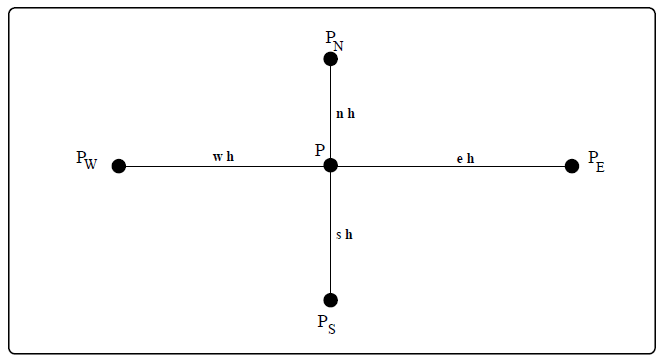
\includegraphics[width=8cm]{./bilder/irregulaereGitter.png}

\end{minipage}
\begin{minipage}{10cm}
$\frac{2}{h^2}(\frac{u(x+eh,y)-u(x,y)}{e(e+w)} +\frac{u(x+wh,y)-u(x,y)}{w(e+w)}
+ \frac{u(x+nh,y)-u(x,y)}{n(n+s)} + \frac{u(x+sh,y)-u(x,y)}{n(n+s)}) = f(x,y)$
\end{minipage}
\subsubsection{Neumann Rand $\delta_n u(x,y) \forall (x,y) \epsilon \delta G$}
\begin{minipage}{8cm}
	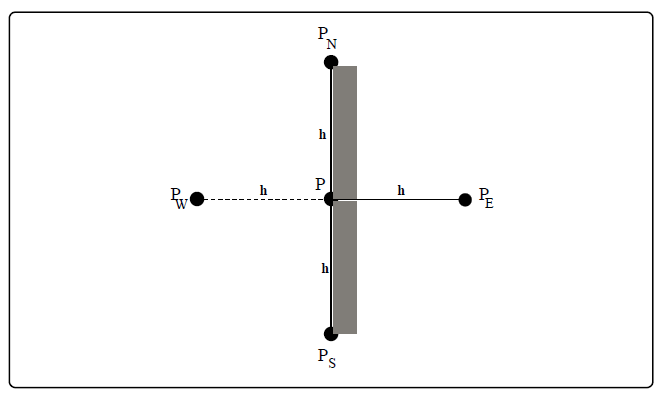
\includegraphics[width=8cm]{./bilder/NeumannRand.png}


\end{minipage}
\begin{minipage}{10cm}
$u(P_W)= u(P_E) - 2 h \delta_x u(P) \Rightarrow $\\
$\frac{2u(P_E) + u(P_N) +
u(P_S)- 4 u(P) - 2h \delta_x u(P)}{h^2}$
\end{minipage}


\subsection{FDM f�r parabolische PDGL}
\subsubsection{explizites Verfahren}
$$\frac{u(x,t+\Delta t) - u(x,t)}{\Delta t} = 
\frac{u(x+\Delta x, t)-2u(x,y) + u( x - \Delta x, t )} {\Delta x^2} $$ 
$$\delta_t
u(x,t)=\delta_{xx}(x,t)$$ 
$ u{j,k+1} = r \tilde{u}{j-1,k} + (1-2r)\tilde{u}{j,k} + r \tilde{u}{j+1,k}
\Longrightarrow$ aus den Positionen k wird k+1 berechtet $r=\frac{\Delta
t}{\Delta x^2}$
Nachteil:\\
$$||A^{-1} < 1 \Longrightarrow \text{um stabiles Verfahren muss} r <
\frac{1}{2}$$
\subsubsection{implizites Verfahren}
$$\frac{u(x,t) - u(x,t -\Delta t)}{\Delta t} = 
\frac{u(x+\Delta x, t)-2u(x,y) + u( x - \Delta x, t )} {\Delta x^2} $$ 
$ u{j,k} = r \tilde{u}{j-1,k+1} + (1+2r)\tilde{u}{j,k+1} + r \tilde{u}{j+1,k+1}
\Longrightarrow
u^{(k)} = E^{(n)} u^{(k+1)}$ Da $||(E^{(n)})^{-1}|| $ immer $< 1$ konvergiert
das implizite Verfahren immer.


\subsubsection{Crank Nicolson -Verfahren (expizite + implezite Verfahren)}


$$ r \tilde{u}{j-1,k+1} + (2+2r)\tilde{u}{j,k+1} + r \tilde{u}{j+1,k+1} = r
\tilde{u}{j-1,k+1} + (2-2r)\tilde{u}{j,k+1} + r \tilde{u}{j+1,k+1} $$

$$
  \begin{bmatrix}
             2-2r& r & 0 & 0\\
             r & 2-2r & r & 0  \\
              0& r &2-2r& r  \\
              0& 0 & r &2-2r \\
             \ldots 
           \end{bmatrix} 
  \begin{bmatrix}
  	T_{1,0}\\
  	T_{2,0}\\
  	T_{3,0}\\
  	T_{4,0}\\
  \end{bmatrix} +
  \begin{bmatrix}
  	T_{0} r\\
  	0\\
  	0\\
  	T_{L} r\\
  \end{bmatrix} = 
  \begin{bmatrix}
             2+2r& -r & 0 & 0\\
             -r & 2+2r & -r & 0  \\
              0& -r &2+2r& -r  \\
              0& 0 & -r &2+2r \\
             \ldots 
           \end{bmatrix} 
  \begin{bmatrix}
  	T_{1,1}\\
  	T_{2,1}\\
  	T_{3,1}\\
  	T_{4,1}\\
  \end{bmatrix} -
  \begin{bmatrix}
  	T_{0} r\\
  	0\\
  	0\\
  	T_{L} r\\
  \end{bmatrix}
  $$
  $\Longrightarrow G^{(n)} u^{(k)} = F^{(n)} u^{(k+1)} \Longrightarrow
  u^{(k+1)}= (F^{(n)})^{-1} G^{(n)} u^{(k)}$

  
  
  
 
\subsection{FDM f�r Hyperbolische PDGL}

$$u_{tt}=u{xx} = homogen$$
$$u_{tt} -u_{xx}= v(x,t) = inhomogen$$

$$\Longrightarrow u_{j,k+1}=r^2 u_{j-1,k} 2(1-r^2)u_{j,k}+ r^2
u_{j+1,k}-u_{j,k-1}$$
\subsubsection{Anfangsbedingungen}
$$\tilde{u}_{j,0} = f(j\Delta x); u_{j,1}= f(j\Delta x) + g(j\Delta x)\Delta t$$
(f(x)= Anfangsfunktion; g(x)=Ableitung; $r = \frac{\Delta t}{\Delta x}$)

\subsubsection{Transportgleichung}
$$u_x(x,t) + u_t(x, t) = 0; u(x,0)=P(x-t)$$
$$\frac{u(x,t+\Delta t)-u(x,t)}{\Delta t} = \frac{u(x,t) - u(x-\Delta x,
t)}{\Delta x}$$

\newpage


\end{document}
